\chapter{Results}
\section{Content Analysis Results}
From the retrospective reports we obtained several interesting results. We will go through each of them below starting with some key numbers and then move on to the results of the content analysis. Then we identify some trends observed while performing the content analysis. 

\subsection{Key Numbers}
In this section we will present some key numbers of the retrospective results and this numbers can also be seen in \autoref{table:key-numbers}.

\begin{table}[!h]
	\begin{center}
	\caption{Some key numbers from the retrospectives}
	\label{table:key-numbers}
	\makebox[\textwidth]{%
		\begin{tabular}{ l | p{0.5\textwidth}}
		\hline
		Key-value & Value  \\
		\hline
		Retrospective report period & 278 Weeks \\
		Number of total actions & 343 \\
		Number of unresolved actions & 65 \\
		Average actions per week & 1.23 \\
		Average unresolved action per week & 0.23 \\
		\hline
		\end{tabular}
	}
\end{center}
\end{table}

The retrospective reports spanned over a period of five years from August 2009 to November 2014. This is equal to 278 weeks and we are going to refer to week numbers from the first retrospective for the remainder of this report. 
During the 278 weeks 77 retrospectives were held and and within these 343 actions was created, where 65 of these actions were still unresolved. This yields an average of 4.45 actions per retrospective and 0.84 unresolved per retrospective. This is equal to 1.23 actions per week, where one have 0.23 unresolved actions per week. 

\begin{sidewaysfigure}[!h]
	\centering
	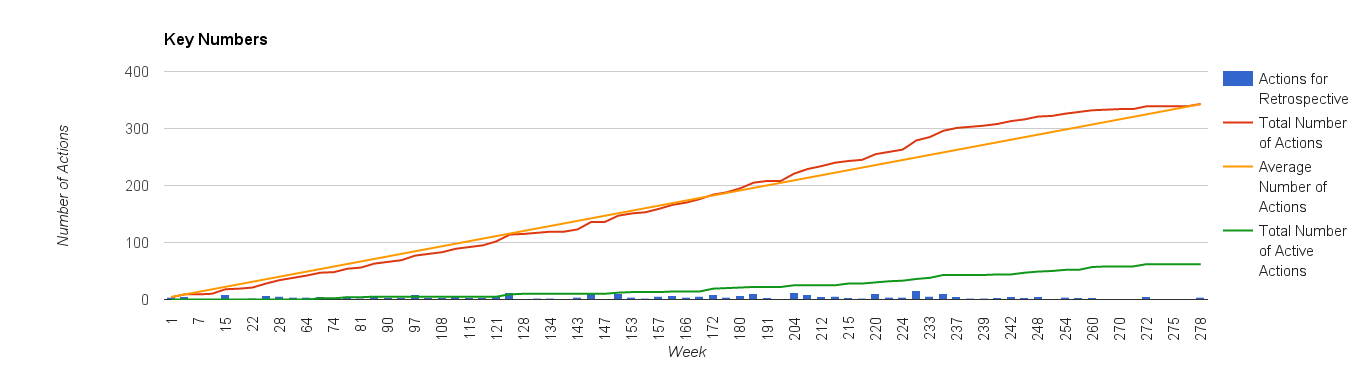
\includegraphics[width=\textwidth]{figures/key-numbers.png}
	\caption{A visual representation of some of the key numbers.}
	\label{figure:key-numbers}
\end{sidewaysfigure}
\afterpage{\clearpage}

In \autoref{figure:key-numbers} we can see the development of numbers of actions. We can see that the team has had a pretty steady amount of actions with no abnormal spikes or changes. The total amount of actions follows the average expected actions quite close and reveals the steady number of actions. The amount of active (or unresolved) actions also has a steady amount of total actions increasing at about the same rate as the total number of actions. 

\subsection{Analysis Results}
In this section we will present the results from our content analysis. We will present the results for each theme defined in \autoref{method:categories}. 

\subsubsection{Nature}

\begin{table}[!h]
	\begin{center}
	\caption{Analysis results from the content analysis for the nature of the action.}
	\label{table:nature-results}
	\makebox[\textwidth]{%
		\begin{tabular}{| l | l | l | l | l |}
		\hline
		Category & \multicolumn{2}{|c|}{All Actions} & \multicolumn{2}{|c|}{Active Actions}  \\
		\cline{2-5}
		& Number & Percentage & Number & Percentage \\	
		\hline
		Positive & 19 & 5.5\% & 1 & 1.6\% \\
		Negative & 310 & 89.3\% & 57 & 90.5\% \\
		Undefined & 18 & 5.2\& & 5 & 7.9\% \\
		\hline
		\end{tabular}
	}
	\end{center}
\end{table}

\begin{table}[!h]
	\begin{center}
	\caption{Analysis results from the content analysis for the context of the action.}
	\label{table:context-results}
	\makebox[\textwidth]{%
		\begin{tabular}{| l | l | l | l | l |}
		\hline
		Category & \multicolumn{2}{|c|}{All Actions} & \multicolumn{2}{|c|}{Active Actions}  \\
		\cline{2-5}
		& Number & Percentage & Number & Percentage \\	
		\hline
		Technical & 157 & 40.4\% & 37 & 52.1\% \\
		Process & 228 & 58.6\% & 34 & 47.9\% \\
		Undefined & 4 & 1\% & 0 & 0\% \\
		\hline
		\end{tabular}
	}
	\end{center}
\end{table}

\begin{table}[!h]
	\begin{center}
	\caption{Analysis results from the content analysis for the decision making perspective of the action.}
	\label{table:decision-making-results}
	\makebox[\textwidth]{%
		\begin{tabular}{| l | l | l | l | l |}
		\hline
		Category & \multicolumn{2}{|c|}{All Actions} & \multicolumn{2}{|c|}{Active Actions}  \\
		\cline{2-5}
		& Number & Percentage & Number & Percentage \\	
		\hline
		Strategic & 55 & 16\% & 10 & 16.1\% \\
		Tactical & 89 & 25.9\% & 18 & 29\% \\
		Operational & 195 & 56.9\% & 33 & 53.2\% \\
		Undefined & 4 & 1.2\% & 1 & 1.6\% \\
		\hline
		\end{tabular}
	}
	\end{center}
\end{table}

\begin{table}[!h]
	\begin{center}
	\caption{Results from the content analysis regarding the organizational learning nature of the action.}
	\label{table:organizational-learning-results}
	\makebox[\textwidth]{%
		\begin{tabular}{| l | l | l | l | l |}
		\hline
		Category & \multicolumn{2}{|c|}{All Actions} & \multicolumn{2}{|c|}{Active Actions}  \\
		\cline{2-5}
		& Number & Percentage & Number & Percentage \\	
		\hline
		Single-loop & 227 & 66.4\% & 41 & 66.1\% \\
		Double-loop & 93 & 27.2\% & 16 & 25.8\% \\
		Undefined & 22 & 6.4\% & 5 & 8.1\% \\
		\hline
		\end{tabular}
	}
	\end{center}
\end{table}

\begin{table}[!h]
	\begin{center}
	\caption{Results from the content analysis in which development phase the action regards.}
	\label{table:development-results}
	\makebox[\textwidth]{%
		\begin{tabular}{| l | l | l | l | l |}
		\hline
		Category & \multicolumn{2}{|c|}{All Actions} & \multicolumn{2}{|c|}{Active Actions}  \\
		\cline{2-5}
		& Number & Percentage & Number & Percentage \\	
		\hline
		Development & 89 & 18.4\% & 11 & 13.1\% \\
		Testing & 102 & 21.1\% & 18 & 21.4\% \\
		Documentation & 64 & 13.2\% & 16 & 19\% \\
		Release & 18 & 3.7\% & 4 & 4.8\% \\
		Build & 23 & 4.8\% & 6 & 7.1\% \\
		Business Development & 18 & 3.7\% & 5 & 6\% \\
		Planning & 119 & 24.6\% & 19 & 22.6\% \\
		Bugfix & 20 & 4.1\% & 2 & 2.4\% \\
		Undefined & 31 & 6.4\% & 3 & 3.6\% \\
		\hline
		\end{tabular}
	}
	\end{center}
\end{table}

\begin{table}[!h]
	\begin{center}
	\caption{Results from the content analysis regarding the collaboration influences of an action.}
	\label{table:collaboration-results}
	\makebox[\textwidth]{%
		\begin{tabular}{| l | l | l | l | l |}
		\hline
		Category & \multicolumn{2}{|c|}{All Actions} & \multicolumn{2}{|c|}{Active Actions}  \\
		\cline{2-5}
		& Number & Percentage & Number & Percentage \\	
		\hline
		Communication & 128 & 35.2\% & 14 & 20.9\% \\
		Leadership & 4 & 1.1\% & 1 & 1.5\% \\
		Competence & 25 & 6.9\% & 1 & 11.9\% \\
		External relations & 42 & 11.5\% & 11 & 16.4\% \\
		Undefined & 185 & 45.3\% & 33 & 48.3\% \\
		\hline
		\end{tabular}
	}
	\end{center}
\end{table}

\afterpage{\clearpage}